\documentclass[a4paper]{article}
%\usepackage{amsfonts}
\usepackage{amsmath}
%\usepackage{amsthm}
\usepackage[utf8]{inputenc}
%\usepackage{hyperref}
%\usepackage{booktabs}
%\usepackage{indentfirst}
\usepackage{graphicx}
%\usepackage{subfig}

\graphicspath{{fig/}}

\title{Fun with Pong}
\author{Cédric Bhihe and Rodrigo Arias}
\date{\today}

% Useful vectorial and matrix notation
\newcommand*\mat[1]{ \begin{pmatrix} #1 \end{pmatrix}}
\newcommand*\arr[1]{ \begin{bmatrix} #1 \end{bmatrix}}
\newcommand*\V[1]{ \boldsymbol{#1}}

\begin{document}
\maketitle

\section{Graphical parts}

A detailed description of the graphical parts of the game is shown in the 
figure~\ref{fig:parts}. The screen holds the surface that can be drawn. Inside, 
the board limits the area where the ball can move. The size of the board cannot 
exceed the screen, but it may be the same size.

\begin{figure}[h]
	\centering
	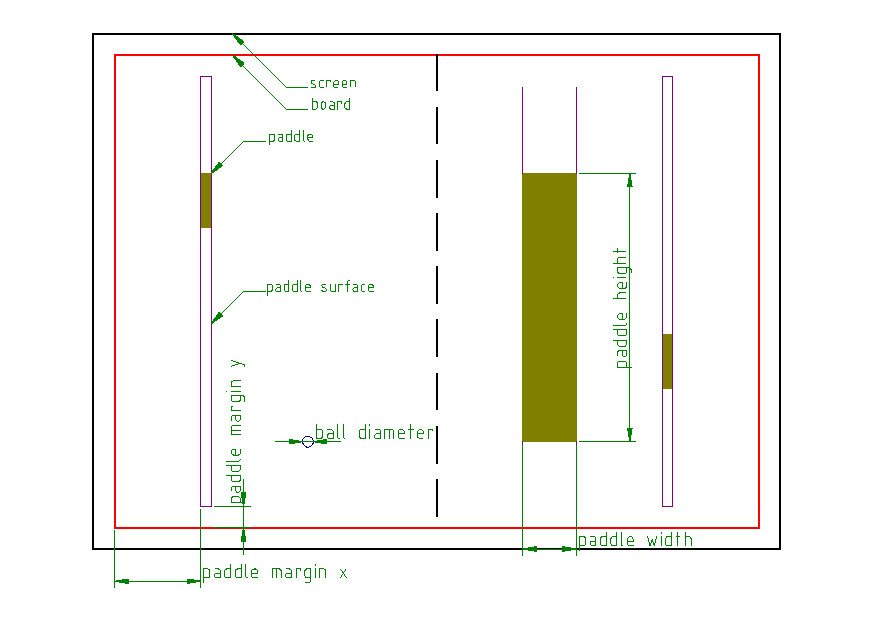
\includegraphics[width=\textwidth]{parts.pdf}
	\caption{Graphical parts of the game.}
	\label{fig:parts}
\end{figure}

The two paddles can be moved inside the paddle surface, but only in the vertical 
axis. A small vertical margin can be left between the paddle surface and the 
board, so the paddles cannot cover the whole board. The horizontal margin is 
only for aesthetic reasons, in order to show the ball falling behind the paddle.

The paddle height and the ball diameter have to be carefully chosen to allow a 
human player to play comfortably, as well as the board and margin dimensions.

\end{document}
